\documentclass[12pt]{article}
\usepackage{setspace}
\usepackage{hyperref}
\usepackage{graphicx}
\graphicspath{ {images/} }
\onehalfspacing
\parskip=2ex
\parindent=2em
\title{Evaluation of MetaEdit+ for DSM}
\author{Jui Deshpande, Sam Minns, Glen Peek}
\date{\today}
\begin{document}
\maketitle
%Optional abstract
\begin{abstract}
In software engineering, there are many approaches for handling the kind of complexities that emerge during development.  One such approach is the use of domain-specific languages within the context of model driven development.  As model driven development has become increasingly popular, new tools have emerged with the aim of allowing users to quickly, easily, and effectively create domain-specific languages.  However, these tools are still far from mainstream.  In this paper, we critique the usability of one such metacase tool, MetaEdit+, by defining a domain-specific language for a library system, describing the creation of this language using MetaEdit+, and reviewing our final result.  
\end{abstract}
\section{Introduction}
The term Domain-Specific Language (DSL) is heard a lot nowadays. A DSL is a language developed to address the need of a given domain. This domain can be a problem domain (e.g. insurance, healthcare, transportation) or a system aspect (e.g. data, presentation, business logic, work flow).
The idea is to have a language with limited concepts which are all focused on a specific domain and describe a meta model therein. \cite{karsai2014design}
This allows teams to focus development efforts on accurately and effectively describing the domain space as opposed to being caught up in low level implementation details.\par
Enhanced focus leads to higher level expressions of the model improving developer productivity and communication with domain experts. The inherent complexity and propensity for error with requirements specifications and analysis is reduced.
In a lot of cases it is even possible to let domain experts use the DSL and develop applications. The combination of these elements leads to more flexible and robust applications that better serve their intended user base.

In this project we created a Domain Specific Language for a simple library management system. We used a meta case modelling tool called MetaEdit+.  The solution consists of some basic building blocks, such as books, authors, librarians. The system describes the appropriate relationships between these entities and the required constraints to ensure the system functions as expected and intended.
\section{Language Design Background}
Despite the lengthy history and recent popularity of domain-specific languages, the task of actually
designing DSLs remains a difficult and under-explored problem~\cite{erwig2014semantics}.

People find DSLs valuable because a well-designed DSL can be much easier to program with than a traditional library. This improves programmer productivity, which is always valuable. In particular it may also improve communication with domain experts, which is an important tool for tackling one of the hardest problems in software development.
Traditionally, the definition of a language proceeds from syntax to semantics. That is, first a syntax is
defined, then a semantic model is decided upon, and finally the syntax is related to the semantic model. 

\subsection{Benefits of DSLs}
Using DSLs can reap a multitude of benefits. 

Once you’ve got a language and its execution engine for a particular aspect of your development task, work becomes much more efficient, simply because you don’t have to do the grunt work manually. 
Using DSLs can increase the quality of the created product: fewer bugs, better architectural conformance, increased maintainability.
Since DSLs capture their respective concern in a way that is not cluttered with implementation details, DSL programs are more semantically rich than GPL programs.
DSLs whose domain, abstractions and notations are closely aligned with how domain experts (i.e. non-programmers), this allows for very good integration between developers and domain experts: domain experts can easily read, and often write program code, since it is not cluttered with implementation details irrelevant to them~\cite{voelter2013dsl}.
\section{MetaEdit+}
With MetaEdit+ an experienced developer defines a domain specific language containing the domain’s concepts and rules in a metamodel, and specifies the mapping from that to code in a domain-specific code generator. For the modeling language implementation, MetaEdit+ provides a metamodeling tool suite for defining the language concepts, rules, symbols, checking reports and generators. Next to the user’s guide, developers are able to watch several webcasts, read articles, blogs, brochures and even listen to podcasts. Generally, Metacase provides really good and clear documentation, but some points could certainly be refined.

Documentation provided
MetaEdit+ offers various DSM resources. This includes a detailed Workbench User’s Guide which discusses every aspect of metamodeling in MetaEdit+. All methods provided by the API are described as well. A single point of criticism in the guide is the rather brief explanation of the API methods and the few examples it delivers.
\section{Library Language}
The Domain Specific Language we have created is an attempt at modelling a Library. We have a chosen the context of a public library as opposed to a specialised facility such as a university or law library. The DSL is naturally constrained by our development tool and as such  is comprised of three main entities. Objects represent physical entities such as loanable items, library equipment and people such as library users and employees. Relationships describe methods by which objects within the DSL may interact. Roles define constraints on the types of objects that may mutually INHABIT? TAKE THE PLACE IN THE RELATIONSHIP, ?BE?, ?RESIDE? word please  end of a relationship between those objects. Additionally constraints may be defined surrounding the semantics of relationships. These constraints fall into four categories:
Connectivity: cardinality and type of some shit about the thing with a thing. 
Occurrence: constraint surrounding the number of a unique objects may appear in a graph
Uniqueness: uniqueness constraints for property values such as ID etc
Port: No fucking idea what the shit port was for, probably something to do with ships.
Creating and applying constraints allows further development and enrichment of DSL semantics.  
\subsection{Objects}
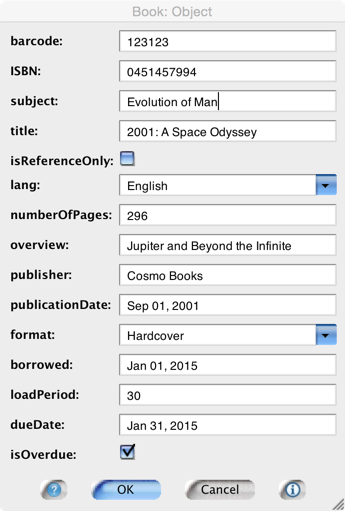
\includegraphics[width=0.5\textwidth]{obj_book}
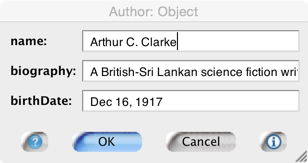
\includegraphics[width=0.5\textwidth]{obj_author}
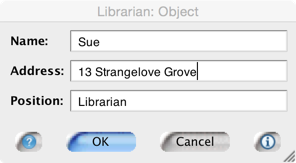
\includegraphics[width=0.5\textwidth]{obj_librarian}
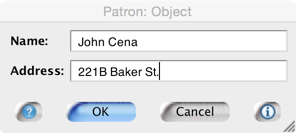
\includegraphics[width=0.5\textwidth]{obj_patron}

\subsection{Relationships/Roles}
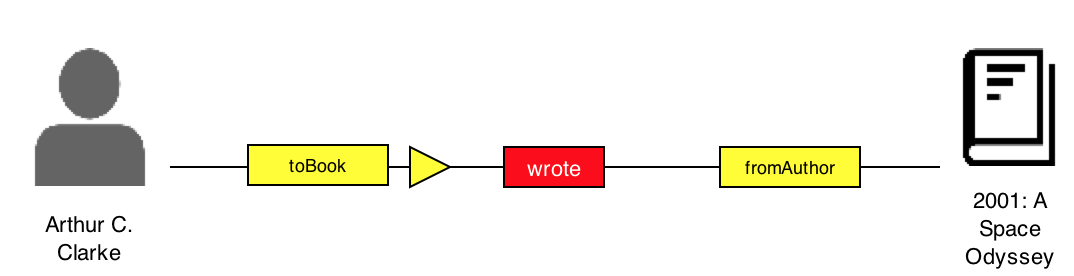
\includegraphics[width=0.5\textwidth]{rel_wrote}
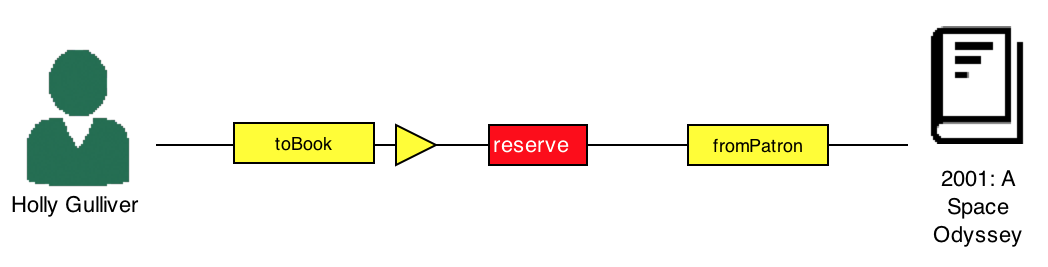
\includegraphics[width=0.5\textwidth]{rel_reserve}
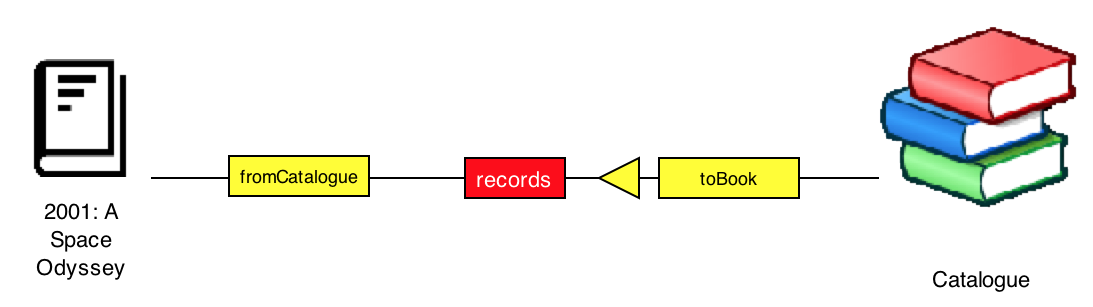
\includegraphics[width=0.5\textwidth]{rel_records}
\subsection{Abstract Syntax}
\section{Discussion}
This section will detail our process of meta modelling tool selection and the reasons for rejecting alternatives. We will discuss and critique the strengths and weaknesses of our selected tool and how these influenced our development process.\par
\subsection{Tool Selection}
We undertook an initial survey both of the tools recommended to us and those identified through literature review and independent research. Of the solutions we found only a small number were still available and even fewer suitable for our project.\par
We rejected a number of tools such as GME due to platform limitations. These tools were only usable within a Windows environment which was unsuitable for our team. Other alternatives such as DOME were rejected due to no longer being maintained and thus unavailable. AtomPM was no longer being maintained and was dependent on legacy versions of NPM packages which rendered it unable to be installed, unstable and unusable.\par Eclipse plugin tools such as Marama and XMF similarly were dependent on legacy versions of Eclipse IDE. The Marama modelling tool was `end of lifed' in 2012 which had the consequence of non existent support or help resources. XMF is no longer maintained and is currently not supported in any modern version of Eclipse and while XMF will load, it no longer functions in any usable way. \par
Other meta modelling tools are available, however, the majority require a licence to be purchased in order to access any meaningful functionality. With these factors in mind we selected to use the only remaining option which was MetaEdit+. 

\subsection{Critique}
During our use of MetaEdit+ we encountered a number of limitations that complicated our development processes. Specifically the limited functionality available through the evaluation license significantly reduced our efficiency as a team. In order to work effectively as a group a concurrent working environment is imperative.\par
In MetaEdit+ team collaboration functionality is limited to paid licenses. In an effort to circumvent this limitation we attempted to implement a GIT work flow, however, as the files used by MetaEdit+ to maintain a project are binaries this was unsuccessful. Had we been able to work concurrently and collaboratively our work flow would have been considerably smoother and more productive.\par
MetaEdit+ uses a kind of version control work flow internally, using the concept of repositories and commits to manage the development of a model. Had we been able to take advantage of this the learning and prototyping phase might have yielded more in the way of usable artefacts. As it transpired the majority of our learning and prototyping artefacts were unusable as the merging of projects was something our licence did not allow.

The way in which DSL elements and the roles and relationships between them are declared is seemingly disconnected from the primary method made available for visualizing the DSL. Similarly the workflow of creating an object, developing relationships and roles between that and existing objects is complex and to a degree opaque. The interface for creating objects, relationships and roles is shown in Figure~\ref{fig:objcreate} is reasonably clear and concise, however, the connections between these parts are not. 

\begin{figure}
  \centering
  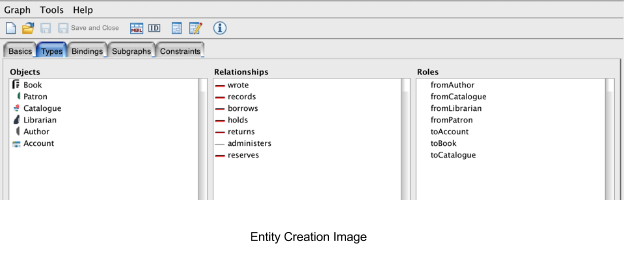
\includegraphics[width=0.8\textwidth]{images/entity_creation.png}
  \caption{The Meta Edit+ entity creation interface.}
  \label{fig:objcreate}
\end{figure}

Relationships and Roles must then be \emph{bound} to Objects. The interface for this process is less clear as shown in Figure~\ref{fig:bindings}. The intuition here is that relationships are bound to a pair of objects via a single role. The reality is that a role is required to describe each end of a relationship between Objects. \par

  \begin{figure}[h]
    \centering
    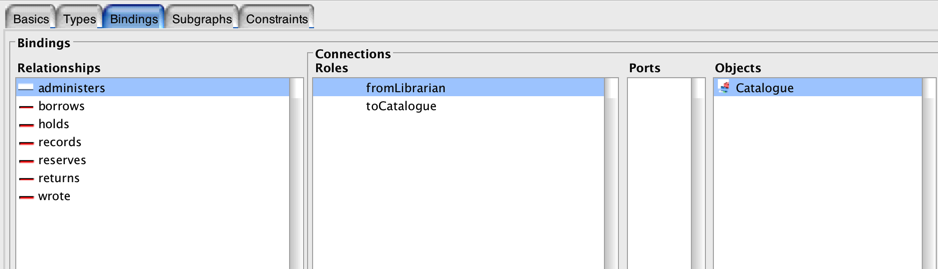
\includegraphics[width=0.8\textwidth]{images/bindings.png}
    \caption{The Meta Edit+ bindings dialogue.}
    \label{fig:bindings}
  \end{figure}

Further complicating this process is the work flow between the graph representation and the bindings declarations. Relationships, roles and the bindings therein are not editable or definable through the graph interface. To define or redefine properties of a relationship or role you are required to exit the \emph{graph view}, enter the \emph{graph tool}, navigate to the bindings window, make the necessary edits and reverse these prior steps to view the result of you action. This makes the process of refining a DSL somewhat arduous and time consuming.\par The provision of editing functionality through the graph view directly would make the process considerably faster and additionally speak more eloquently to the connection between a language element and its representation.\par
Communication to the user concerning the Meta Edit+ internal syntax could be more effective.
The error messages that propagate through the graph interface are indistinct and open to interpretation. They offer little in the way of detail or guidance, functioning more to alert the user to having done something wrong rather than how that might be rectified as shown in Figure~\ref{fig:error}. \par

  \begin{figure}[h]
    \centering
    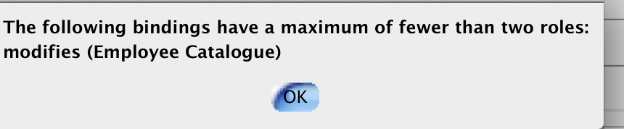
\includegraphics[width=0.8\textwidth]{images/entity_error.png}
    \caption{Graph interface error messages can be difficult to interpret.}
    \label{fig:error}
  \end{figure}

The final limitation of Meta Edit+ was its inability to easily produce Transformations.  It does have the ability to use SOAP, Web Services, or a .NET API to transform your DSM to testing tools or to Models in other tools.  The easiest way to accomplish a transformation for a new user is to use MetaEdit+'s built in Generator option.  This allows a user to do simple transformations in that one can analyse / generate reports about their DSL and currently modelled implementation.\par 
In our case, we are able to check whether a modeller using our DSL has met the requirements of our system.  We created a Test Script object that had a Test list.  Modellers can choose which test to run, or simply run all of the tests as shown in Figure~\ref{fig:transform_script}.\par

  \begin{figure}[h]
    \centering
    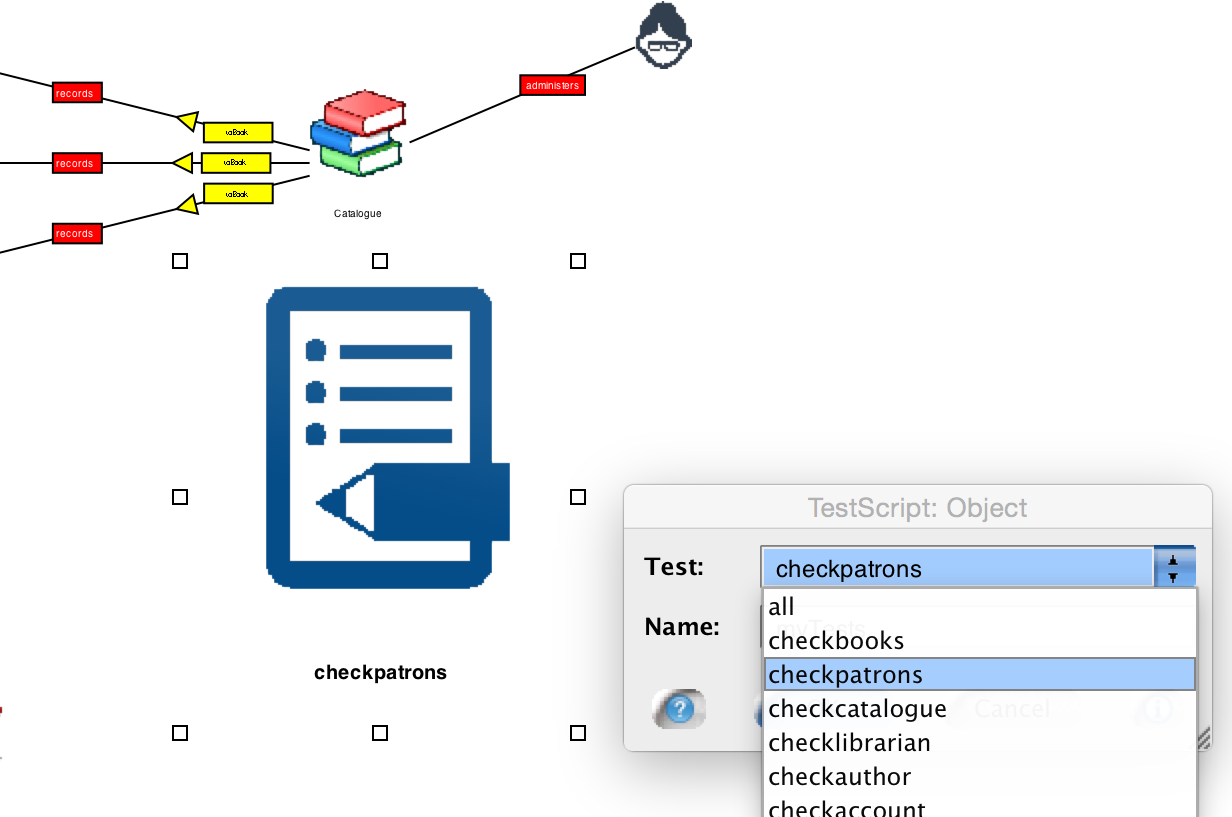
\includegraphics[scale=0.3]{images/transform_script.png}
    \caption{Users can select which Model Validation tests they would like to run.}
    \label{fig:transform_script}
  \end{figure} 
  
When a Test Script is present in the model and a test has been selected, the modeller may then choose to run the Generator Validate Model (Figure~\ref{fig:transform_code}).\par
  \begin{figure}[h]
    \centering
    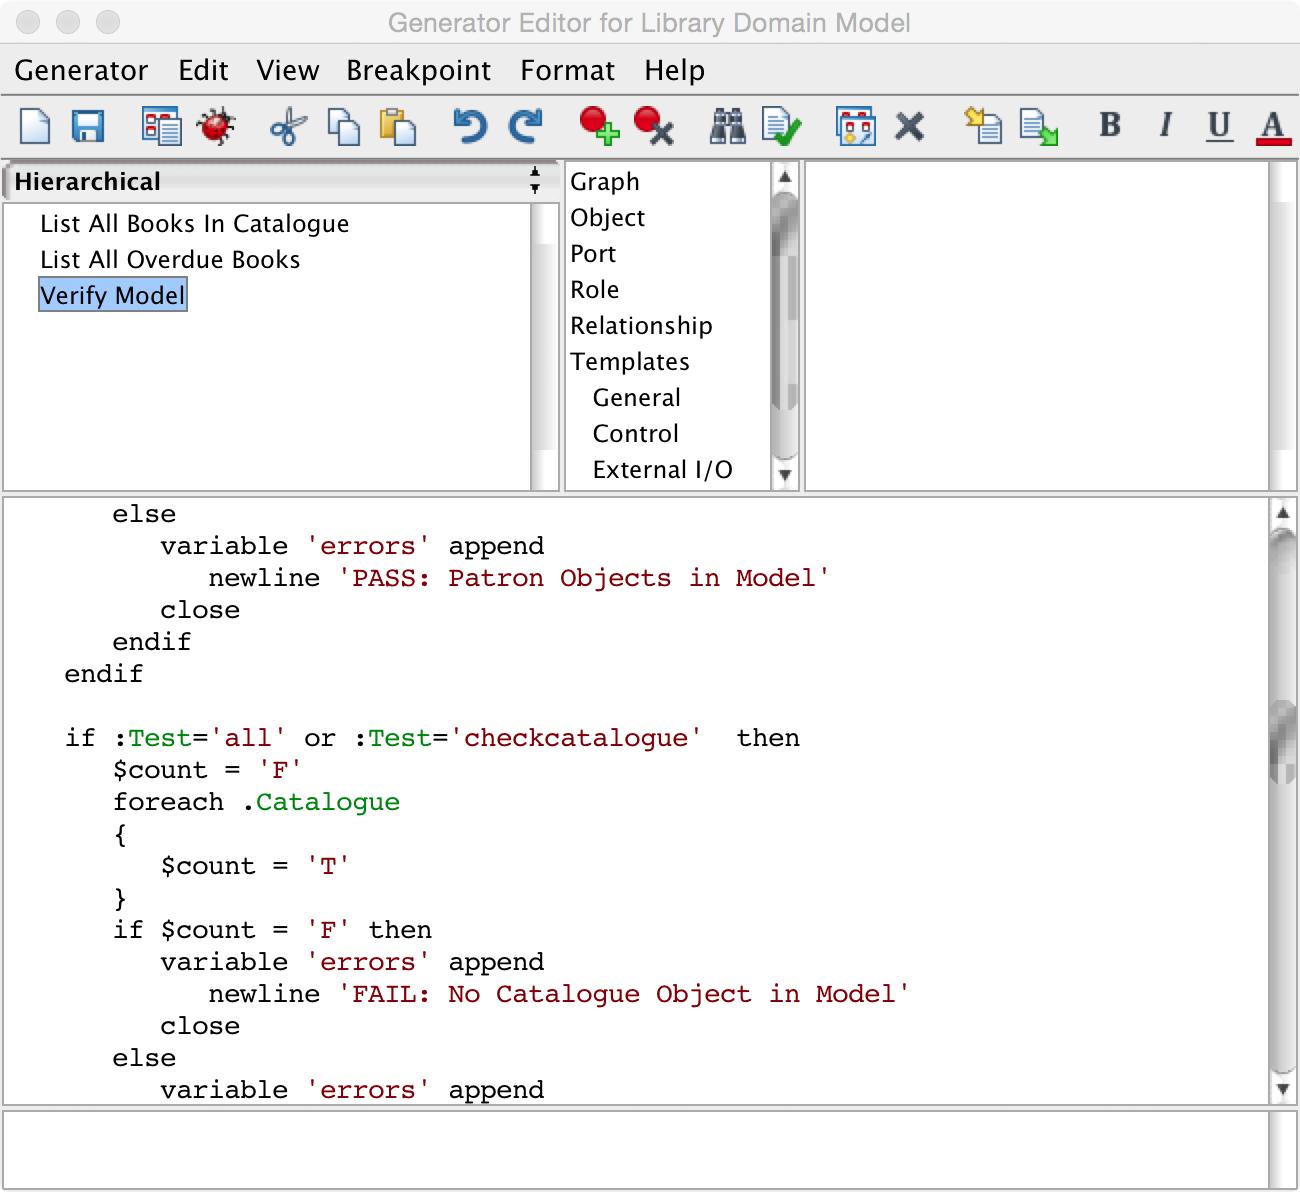
\includegraphics[scale=0.3]{images/transform_code.png}
    \caption{Validate Model Generator}
    \label{fig:transform_code}
  \end{figure} 
Validate Model then runs through the user created model and checks whether there are appropriate instances of each type of object, whether each object has appropriate relationships, and whether there are any disconnected objects that are either unnecessary or have been overlooked in the implementation of the library system.  The results of these tests are output to a report that tells the user whether there model meets the criteria for being a proper library model as you can see in Figure~\ref{fig:transform_report}.\par
  \begin{figure}[h]
    \centering
    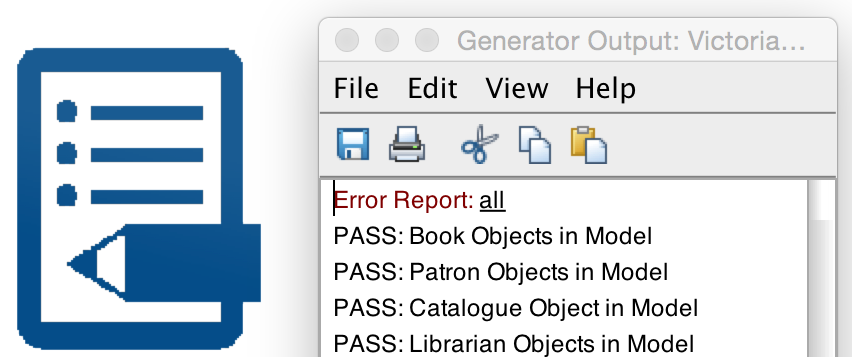
\includegraphics[scale=0.3]{images/transform_all.png}
    \caption{Validate Model Generator Report}
    \label{fig:transform_report}
  \end{figure} 

In contrast to some of the negative aspects of the interface design and work flow issues Meta Edit+ did have some advantages.

MetaEdit+ provides cross platform support, this means that team members are not limited to one platform, and can choose to create DSL’s on their platform of choice. This is in contrast to solutions mentioned earlier in this section that only supported Windows environments. \par

Another major advantage in MetaEdit+ was its community. The MetaEdit+ forums are fairly active and one could expect an answer to any question within a reasonable time frame.  We also found, even in our trial version, that the development team themselves were all too happy to help. Their support staff pre-emptively email users offering help and guidance in the use of their tool.


\section{Conclusion}
Our initial investigation into MetaEdit+ seemed to suggest that it was an ideal tool for our purposes.  However, we quickly learned that the overall work flow of MetaEdit+ has a steep learning curve.  As we progressed, the work flow did become easier, but this was only with research, practice, and time.  While experts may find this tool incredibly handy, novices will continue to struggle as it hasn't quite made the process intuitive.  MetaEdit+ shows a lot of promise, and although it has been around for years, it still has not quite cracked the winning formula.
\bibliographystyle{acm}
\bibliography{mybib}
\end{document}
  